\documentclass[12pt]{report}

\usepackage[utf8]{inputenc}
\usepackage[smartEllipses]{markdown}
\usepackage{minted}

\usepackage{graphicx}
\graphicspath{{../img/}}

\usepackage{hyperref}
\hypersetup{
	colorlinks = true,
	linkcolor = blue,
	filecolor = magenta,      
	urlcolor = cyan,
}

\urlstyle{same}

\newcommand{\newpar} {
    \vskip 1cm
}

\title{SVMs applied to DoS Attack Detection}
\author{David Carrascal, Adrián Guerrero, Artem Strilets, Pablo Collado}
\date{January 2020}

\begin{document}

	\begin{titlepage}
		\maketitle
	\end{titlepage}

	\begin{abstarct}
		The purpose of this project is to develop an artificial intelligence to classify possible DDoS attacks in an SDN network. This will be done by using data collectors such as Telegraf, Mininet to emulate the SDN network, and InfluxDB and Grafana as a means to store data and visualize it respectively. For non-English speakers we leave part of the content of this guide written in Spanish:

		\begin{itemize}
			\item Network Scenario - Mininet Guide: \href{https://hackmd.io/@davidcawork/r1fZC-nRS}{Link}
			\item DDoS using hping3 tool Guide: \href{https://hackmd.io/@davidcawork/HJ_D7jA0r}{Link}
			\item Mininet Internals (II) Guide: \href{https://hackmd.io/@davidcawork/SyrwHoNJL}{Link}
		\end{itemize}

		\textbf{Keywords}: \href{https://www.digitalattackmap.com}{\textit{DDoS attacks}}; \href{https://www.opennetworking.org/sdn-definition}{\textit{SDN network}}; \href{https://www.sciencedirect.com/science/article/abs/pii/016974399500050X}{\textit{Artificial Intelligence classification}}; \href{http://mininet.org}{\textit{Mininet}}
	\end{abstarct}

	\tableofcontents

	\section{Notes}
		Throughout the document we will always be talking about 2 virtual machines (VMs) on which we implement the scenario we are discussing. In order to keep it simple we have called one VM \textbf{controller} and the other one \textbf{test}. Even though the names may seem kind of random at the moment we promise they're not. Just keep this in mind as you continue reading.

	\section{Installation Methods}
		We have created a \textbf{Vagrantfile} through which we provide each machine with the necessary scripts to install and configure the scenario. By working in a virtualized environment we make sure we all have the exact same configuration so that tracing and fixing errors becomes much easier. If you do not want to use Vagrant as a provider you can follow the native installation method we present below.

		\subsection{Vagrant}
			First of all, clone the repository from GitHub :octocat: and navigate into the new directory with:

			\begin{minted}{bash}
				git clone https://github.com/GAR-Project/project
				cd project
			\end{minted}

			We power up the virtual machine through \textbf{Vagrant}:

			\begin{minted}{bash}
				vagrant up
			\end{minted}

			And we have to connect to both machines. \textbf{Vagrant} provides a wrapper for the \textit{SSH} utility that makes it a breeze to get into each virtual machine. The syntax is just \texttt{vagrant ssh <machine_name>} where the \texttt{<machine_name>} is given in the \textbf{Vagrantfile} (take a look at the appendix for more details):

			\begin{minted}{bash}
				vagrant ssh test
				vagrant ssh controller
			\end{minted}

			We should already have all the machines configured with all the necessary tools to bring our network up with Mininet on the \textbf{test} VM, and Ryu on the \textbf{controller} VM. This includes every \texttt{python3} dependency as well as any needed packages.

			\subsubsection{Troubleshooting Problems Regarding \texttt{SSH}}
				If you have problems connecting via SSH to the machine, check that the keys in the path \texttt{.vagrant/machines/test/virtualbox/} are owned by the user, and have read-only permissions for the owner of the key. 

				\begin{minted}{bash}
					cd .vagrant/machines/test/virtualbox/
					chmod 400 private_key

					# We could also use this instead of "chmod 400" (u,g,o -> user, group, others)
					# chmod u=r,go= private_key
				\end{minted}

				Instead of using vagrant's manager to make the \texttt{SSH} connection, we can opt for manually doing it ourselves by passing the path to the private key to SSH. For example:

				\begin{minted}{bash}
					ssh -i .vagrant/machines/test/virtualbox/private_key vagrant@10.0.123.2
				\end{minted}

		\subsection{Native}
			This method assumes you already have any VMs up and running with the correct configuration and dependencies installed. Ideally you should have 2 VMs. We will be running \textbf{Ryu} (the \textit{SDN} controller) in one of them and we will have \textbf{mininet}'s emulated network with running in the other one. Try to use Ubuntu 16.04 (a.k.a \textbf{Xenial}) as the VM's distribution to avoid any mistakes we may have not encountered.

			First of all clone the repository, just like how the Kaminoans do it and then navigate into it:

			\begin{minted}{bash}
				git clone https://github.com/GAR-Project/project
				cd project
			\end{minted}

			Manually launch the provisioning scripts in each machine:

			\begin{minted}{bash}
				# To install Mininet, Mininet's dependencies and telegraf. Run it on the "mininet" VM
				sudo ./util/install_mininet.sh
				sudo ./util/install_telegraf.sh

				# To install Ryu and Monitoring system (Grafana + InfluxDB). Run it on the "controller" VM
				sudo ./util/install_ryu.sh
				sudo ./util/install_grafana_influxdb.sh
			\end{minted}

	\section{Our Scenario}
		Our network scenario is described in the following script: \href{https://github.com/GAR-Project/project/blob/master/src/scenario_basic.py}{\texttt{src/scenario_basic.py}}. Mininet makes use of a Python API to give users the ability to automate processes easily, or to develop certain modules at their convenience. For this and many other reasons, Mininet is a highly flexible and powerful tool for network emulation which is widely used by the scientific community.

		\begin{itemize}
			\item For more information about the API, see its \href{http://mininet.org/api/annotated.html}{manual}.
		\end{itemize}

		\begin{figure}
			\centering
			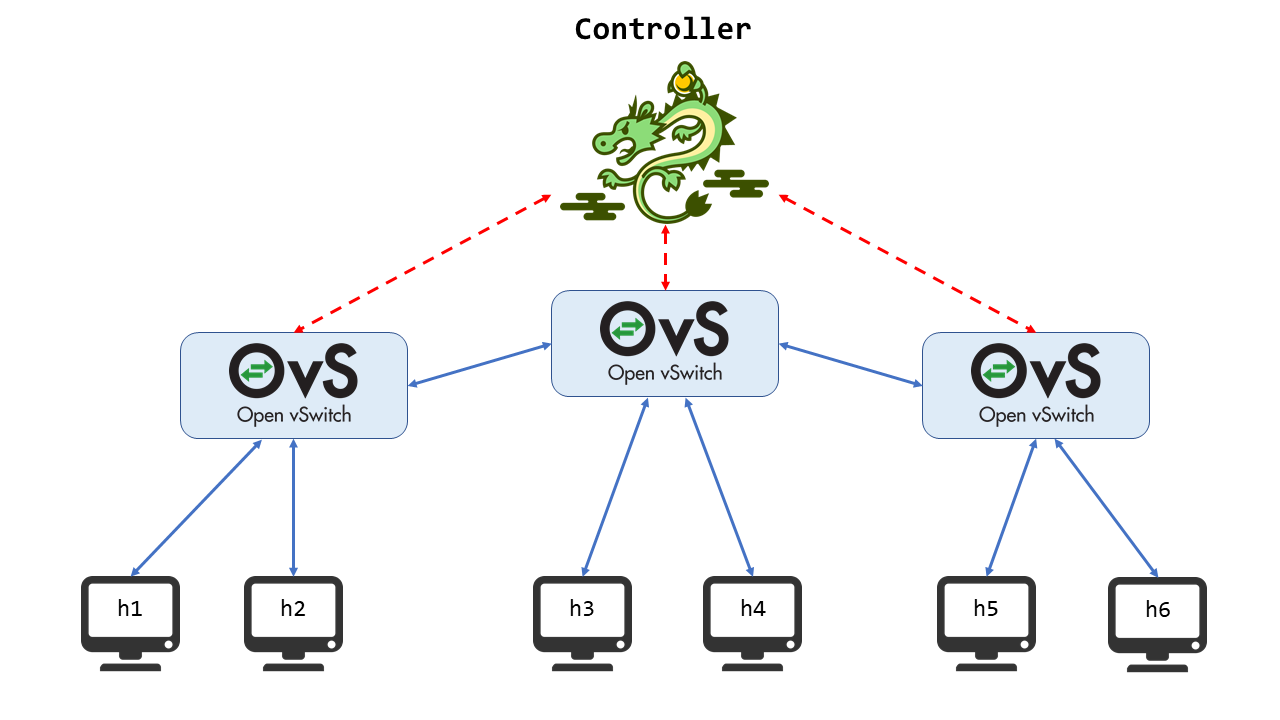
\includegraphics[scale = 1]{scenario.png}
			\caption{Mininet's Scenario}
			\label{f:scenario}
		\end{figure}

		Figure \ref{f:scenario} presents us with the \textit{logic} scenario we will be working with. As with many other areas in networking this logic picture doesn't correspond with the real implementation we are using. We have seen throughout the installation procedure how we are always talking about 2 VMs. If you read carefully you'll see that one VM's "names" are \textbf{controller} and \textbf{mininet}. So it should come as no surprise that the controller and the network itself are living in different machines!
		\newpar
		The first question that may arise is how on Earth can we logically join these 2 together. When working with virtualized environments we will generate a virtual LAN where each VM is able to communicate with one another. Once we stop thinking about programs and abstract the idea of "\textit{process}" we find that we can easily identify the \textbf{controller} which is just a \textbf{ryu} app, which is nothing more than a \textbf{python3} app with the \textbf{controller}'s VM \textbf{IP} address and the port number where the \textbf{ryu} is listening. We shouldn't forget that \textbf{any} process running within \textbf{any} host in the entire \textbf{Internet} can be identified with the host's \textbf{IP} address and the processes \textbf{port} number. Isn't it amazing?
		\newpar
		OK, the above sounds great but... Why should we let the controller live in a machine when we could have everything in a single machine and call it a day? We have our reasons:

		\begin{itemize}
			\item Facilitate teamwork, since the \textbf{AI's logic} will go directly into the controller's VM. This let's us increase both working group's independence. One may work on mininet's core and the data collection with \textbf{telegraf} whilst the other can look into the DDoS attack detection logic and visualization using \textbf{Grafana} and \textbf{InfluxDB}.
			\item Facilitate the storage of data into \textbf{InfluxDB} from \textbf{telegraf}, as due to the internal workings of Mininet there may be conflicts in the communication of said data. Mininet's basic operation at a low level is be detailed below.
			\item Having two different environments relying on distinct tools and implementing different functionalities let's us identify and debug problems way faster. We can know what piece of software is causing problems right away!
		\end{itemize}

		\subsection{Running the scenario}
			Running the scenario requires having logged into both VMs manually or using vagrant's SSH wrapper. First of all we're going to power up the controller, to do so we run the following from the \texttt{controller} VM. It's an application that does a basic forwarding, which is just what we need:

			\begin{minted}{bash}
				ryu-manager ryu.app.simple_switch_13
			\end{minted}

			You might prefer to run the controller in the background as it doesn't provide really meaningful information. In order to do so we'll run:

			\begin{minted}{bash}
				ryu-manager ryu.app.simple_switch_13 > /dev/null 2>&1 &
			\end{minted}

			Let's break this big boy down:

			\begin{itemize}
				\item \texttt{> /dev/null} redirects the \texttt{stdout} file descriptor to a file located in \texttt{/dev/null}. This is a "special" file in Linux systems that behaves pretty much like a black hole. Anything you write to it just "disappears" :open_mouth:. This way we get rid of all the bloat caused by the network startup.
				\item \texttt{2>&1} will make the \texttt{stderr} file descriptor point where the \texttt{stdout} file descriptor is currently pointing (\texttt{/dev/null}). Terminal emulators usually have both \texttt{stdout} and \texttt{stderr}"going into" the terminal itself so we need to redirect these two to be sure we won't see any output.
				\item \texttt{&} makes the process run in the background so that you'll be given a new prompt as soon as you run the command.
			\end{itemize}

			If you want to move the controller app back into the foreground so that you can kill it with \texttt{CTRL + C} you can run \texttt{fg} which will bring the last process sent to the background back to the foreground.

			\begin{figure}
				\centering
				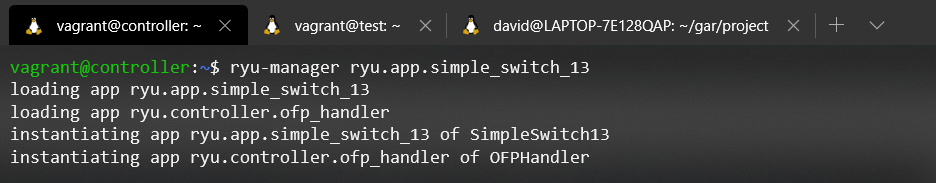
\includegraphics[scale = 1]{controller_ex.png}
				\caption{The controller is now running}
			\end{figure}

			Once the controller is up we are going to execute the network itself, to do so launch the aforementioned script from the \texttt{test} machine:

			\begin{minted}{bash}
				sudo python3 scenario_basic.py
			\end{minted}

			\begin{figure}
				\centering
				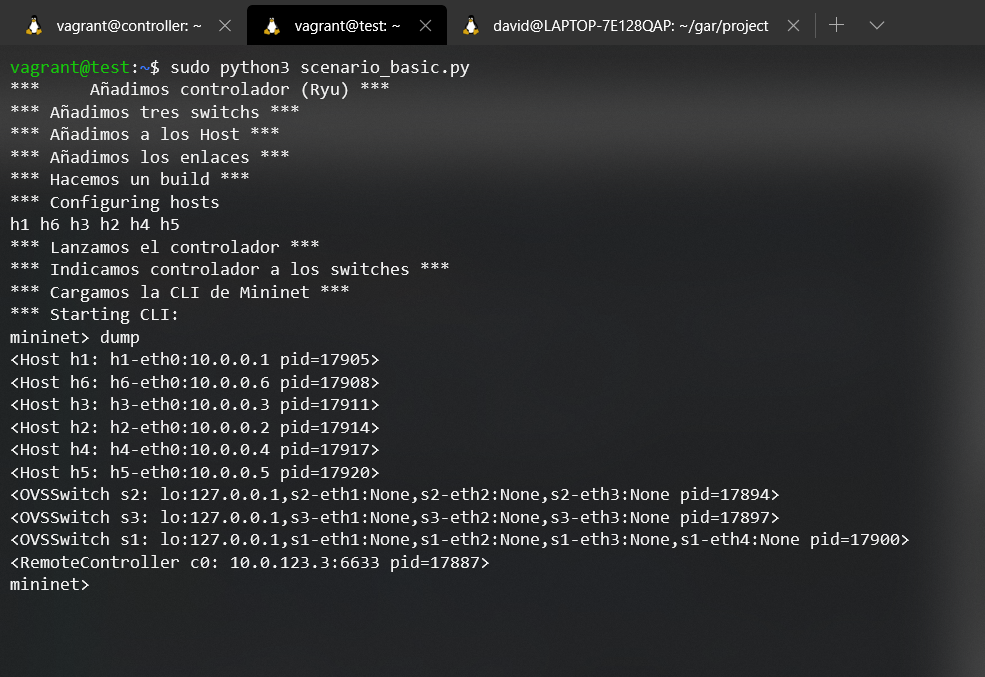
\includegraphics[scale = 1]{mininet_up.png}
				\caption{Mininet is now UP}
				\label{f:mininet_up}
			\end{figure}

			Notice how we have opened \textbf{Mininet CLI} from the \texttt{test} machine in figure \ref{f:mininet_up}. We can perform many actions from this command line interface. The most useful will be detailed below.

		\subsection{Is it working properly?}
			We should have our scenario working as intended by now. We can check our network connectivity by pinging the hosts, for example:

			\begin{minted}{bash}
				mininet> h1 ping h3

				# We can also ping each other with the pingall command
				mininet> pingall
			\end{minted}

			\begin{figure}
				\centering
				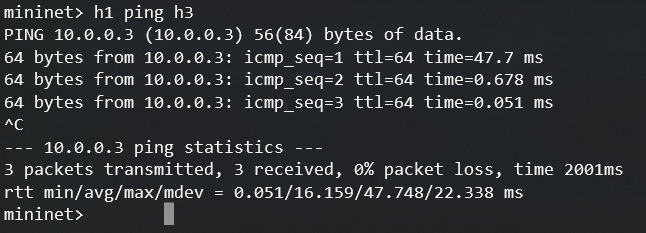
\includegraphics[scale = 1]{ping_ok.png}
				\caption{Mininet is working OK}
				\label{f:ping_ok}
			\end{figure}

			As you can see in figure \ref{f:ping_ok} above, there is full connectivity in our scenario. You may have noticed how the first \textbf{ping} takes way longer than the other to get back to use. That is, its \textbf{RTT} (\textbf{R}ound \textbf{T}rip \textbf{T}ime) is abnormally high. This is due to the empty \textbf{ARP} tables we currently have \textit{AND} to the fact that we don't yet have a flow defined to handle \textbf{ICMP} traffic:

			\begin{itemize}
				\item An \textbf{ARP} resolution between sender and receiver of the ping takes place so that the sender learns the next hop's \textbf{MAC} address.
				\item In addition, the \textbf{ICMP} message (ping-request) will be redirected to the driver (a.k.a controller) to decide what to do with the packet as the switches don't yet have a \textbf{flow} to handle this traffic type. This way the controller will, when it receives the packet, instantiate a set of rules on the switches so that the \textbf{ICMP} messages are routed from one host to the other.
			\end{itemize}

			\begin{figure}
				\centering
				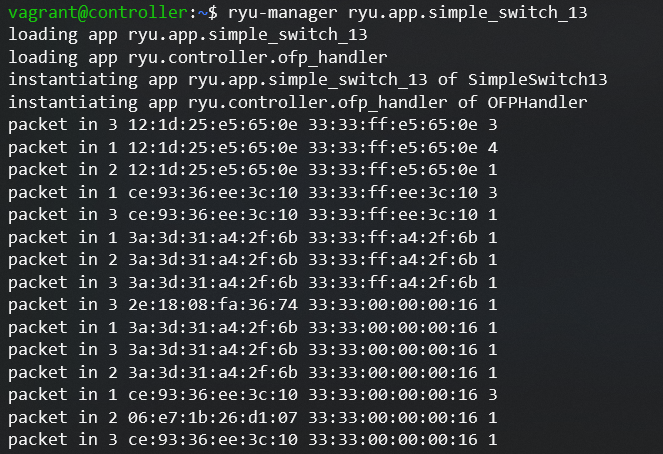
\includegraphics[scale = 1]{ryu_rcv.png}
				\caption{Ryu is configuring the flows}
				\label{f:ryu_rcv}
			\end{figure}

			As you can see in figure \ref{f:ryu_rcv}, the controller's \textbf{stdout} (please see the [appendix](#appendix) to learn more about file descriptors) indicates the commands it has been instantiating according to the packets it has processed. In the end, for the first packet we will have to tolerate a delay due to \textbf{ARP} resolution and \textbf{flow} lookup and instantiation within the controller. The good thing is the rest of the packets will already have the destination \textbf{MAC} and the rules will already instantiated in the intermediate switches, so the new delay will be minimal.

	\section{Attack Time}
		We have already talked about how to set up our scenario but we haven't got into breaking things (i.e the fun stuff :smiling_imp:). Our goal is to simulate a **DoS** (**D**enial **o**f **Service**) attack. Note that we usually refer to this kind of threats as **DDoS** attacks where the first **D** stands for **D**istributed. This second "name" implies that we have multiple machines trying to flood our own. We are going to launch the needed amounts of traffic from a single host so we would be making a mistake if we were talking about a distributed attack. All in all this is just a minor nitpick, the concept behind both attacks is exactly the same.
		\newpar
		We need to flood the network with traffic, great but... How should we do it? We already introduced the tool we are going to be using: **hping3**. This program was born as a TCP/IP packet assembler and analyser capable of generating ICMP traffic. Its biggest asset is being able to generate these ICMP messages as fast as the machine running it can: just what we need :japanese_goblin:.
		\newpar
		The main objective is being able to classify the traffic in the network as a normal or an abnormal situation with the help of AI algorithms. For these algorithms to be effective we need some training samples so that they can "learn" how to regard and classify said traffic. That's why we need a second tool capable of generating "normal" ICMP traffic so that we have something to compare against. Good ol' **ping** is our pal here.

		\subsection{Time To Limit The Links}
			We should no mention our scenario again. We had a **Ryu** controller, three **OVS** switches and several hosts "hanging" from these switches. The question is: **what's the capacity of the network links?**
			\newpar
			According to Mininet's \href{https://github.com/mininet/mininet/wiki/Introduction-to-Mininet}{wiki} that capacity is not limited in the sense that the network will be able to handle as much traffic as the hardware emulating it can. This implies that the more powerful the machine, the larger the link capacity will be. This poses a problem to our experiment as we want it to be reproducible in any host. That's why we have decided to limit each link's bandwidth during the network setup.
			\newpar
			This behaviour is a consequence of Mininet's implementation. We'll discuss it when analyzing mininet's internals later on later down the road but the key aspect is that we cannot neglect Mininet's implementation when making design choices!

			\subsubsection{How To Limit Them}
				In order to limit the available **BW** (**B**and **W**idth) we'll use Mininet's API. This API is just a wrapper for a **TC** (**T**raffic **C**ontroller) who is in charge of modifying the kernel's **planner** (i.e *Network Scheduler*). The code where we leverage the above is:

				\begin{minted}{python}
					net = Mininet(topo = None,
								  build = False,
								  host = CPULimitedHost,
								  link = TCLink,
								  ipBase = '10.0.0.0/8')
				\end{minted}

				Note how we need to limit each host's capacity by means of the CPU which is what we do through the `host` parameter in Mininet's constructor. We'll also need links with a `TCLink` type. We can achieve this thanks to the `link` parameter. This will let us impose the limits to the network capacity ourselves instead of depending on the host's machines capabilities.
				\newpar
				After fiddling with the overall constructor we also need to take care when defining the network links. We can find the following lines over at **src/scenario_basic.py**:

				\begin{minted}{python}
					net.addLink(s1, h1, bw = 10)
					net.addLink(s1, h2, bw = 10)
					net.addLink(s1, s2, bw = 5, max_queue_size = 500)
					net.addLink(s3, s2, bw = 5, max_queue_size = 500)
					net.addLink(s2, h3, bw = 10)
					net.addLink(s2, h4, bw = 10)
					net.addLink(s3, h5, bw = 10)
					net.addLink(s3, h6, bw = 10)
				\end{minted}

				We are fixing a **BW** for the links with the `bw` parameter. We have also chosen to assign a finite buffer size to the middle switches in an effort to get as close to reality as we possibly can. If the `max_queue_size` parameter hadn't been defined we would be working with "infinite" buffers at each switch's exit ports. Having these finite buffers will in fact introduce a damping effect in our tests as once you fill them up you can't push any more data through: the output queues are absolutely full... In a real-life scenario we would suffer huge packet losses at the switches and that could be used as a symptom as well but we haven't taken it into account for the sake of simplicity.
				\newpar
				We fixed the queue lengths so that they were coherent with standard values. We decided to use a **500 packet** size because *Cisco*'s (:satisfied:) queue lengths range from 64 packets to about 1000 as found \href{https://www.cisco.com/c/en/us/support/docs/routers/7200-series-routers/110850-queue-limit-output-drops-ios.html}{here}. We felt like 500 was an appropriate value in the middle ground. With all these restrictions our scenario would look like figure \ref{f:limited}.

				\begin{figure}
					\centering
					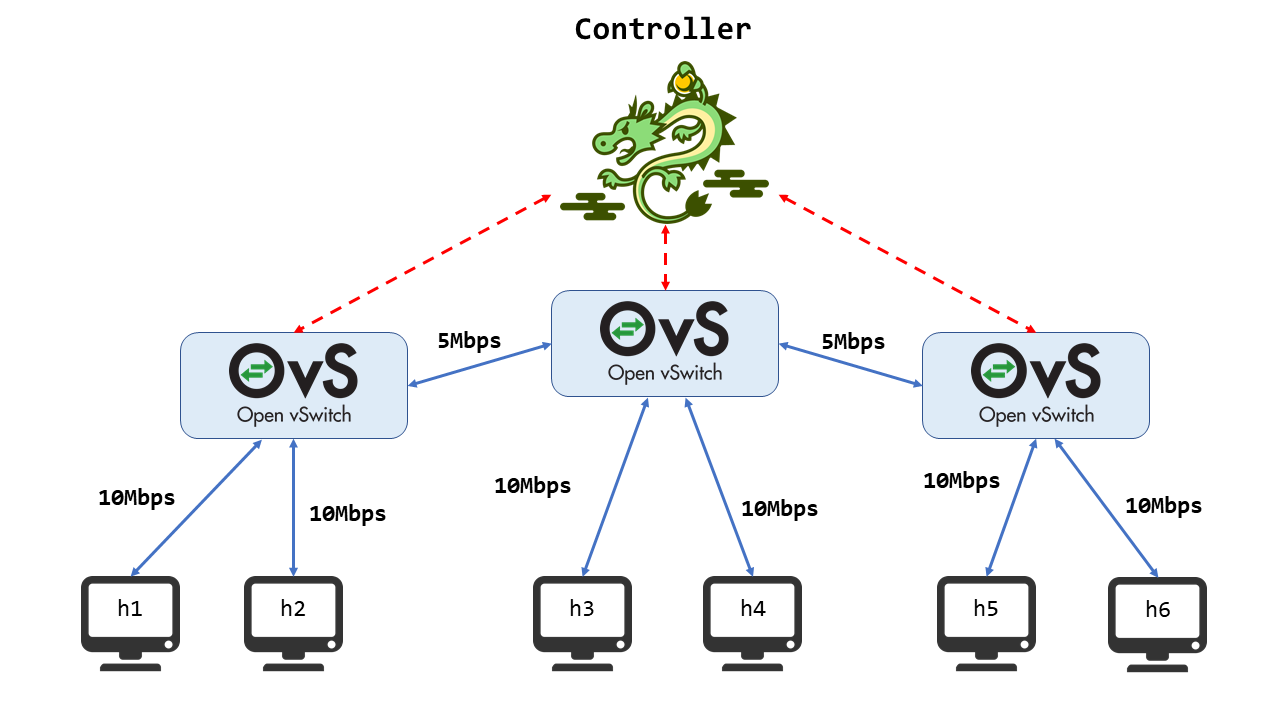
\includegraphics[scale = 1]{scenario_limits.png}
					\caption{Scenario with link capacities}
					\label{f:limited}
				\end{figure}

				By inspecting the network dimensions we can see how we have a clear bottleneck... This "flaw" has been introduced on purpose as we want to clearly differentiate regular traffic from the one we experience when under attack.

		\subsection{Getting Used to \textt{hping3}}
			This versatile tool can be configured so that it can explore a given network, perform traceroutes, send pings or carry out out flood attacks on different network layers. All in all, it lets us craft our own packets and send them to different destinations at some given rates. You can even forge the source **IP** address to go full stealth mode :ghost:. We'll just send regular pings: **ICMP --> Echo request (Type = 8, Code = 0)** whilst increasing the rate at which we send them. This will in turn make the network core collapse making our attack successful.
			\newpar
			Check out this \href{https://tools.kali.org/information-gathering/hping3}{site} for more info on this awesome tool.

		\subsection{Installing Things... Again!}
			The tool will be already present on the test machine as it was included in the **Vagrantfile** as part of the VM's provisioning script. In case you want to manually install it you can just run the command below as **hping3** is usually within the default software sources:

			\begin{minted}{bash}
				sudo apt install hping3
			\end{minted}

		\subsection{Usage}
			As we have previously discussed this is quite a complete tool so we will only use one of the many functionalities to keep things simple. The command we'll be using is:

			\begin{minted}{bash}
				hping3 -V -1 -d 1400 --faster <Dest_IP>
			\end{minted}

			We are going to break down each of the options:

			\begin{itemize}
				\item `-V`: Show verbose output (i.e show more information)
				\item `-1`: Generate ICMP packets. They'll be ping requests by default
				\item `-d 1400`: Add a bogus payload. This is not strictly needed but it'll help us use up the link's BW faster. We have chosen a 1400 B payload so as not to suffer fragmentation at the network layer.
				\item `--faster`: If we used the \textt{flood} option we overwhelmed the virtualized network...
			\end{itemize}

			We would like to point out that `hping3` could have been invoked with the `--flood` option instead of `--faster`. When using `--flood` the machine will generate as many packets as it possibly can. This would be great in a world of rainbows but... The virtual network was quickly overwhelmed by the ICMP messages and packets began to be discarded everywhere. Event though this is technically a **DoS** attack gone right too it obscures the phenomena we are faster so we decided to use `--faster` as the rate it provides suffices for our needs.

		\subsection{Demo Time!}
			The attack we are going to carry out comprises hosts **1**, **2** and **4**. We'll launch `hping3` from **Host1** targeting **Host4** and we'll try to ping **Host4** from **Host2**. We will in fact see how this "regular" ping doesn't get through as a consequence of a successful **DoS** attack. Figure \ref{f:dos_atk} depicts the situation.

			\begin{figure}
				\centering
				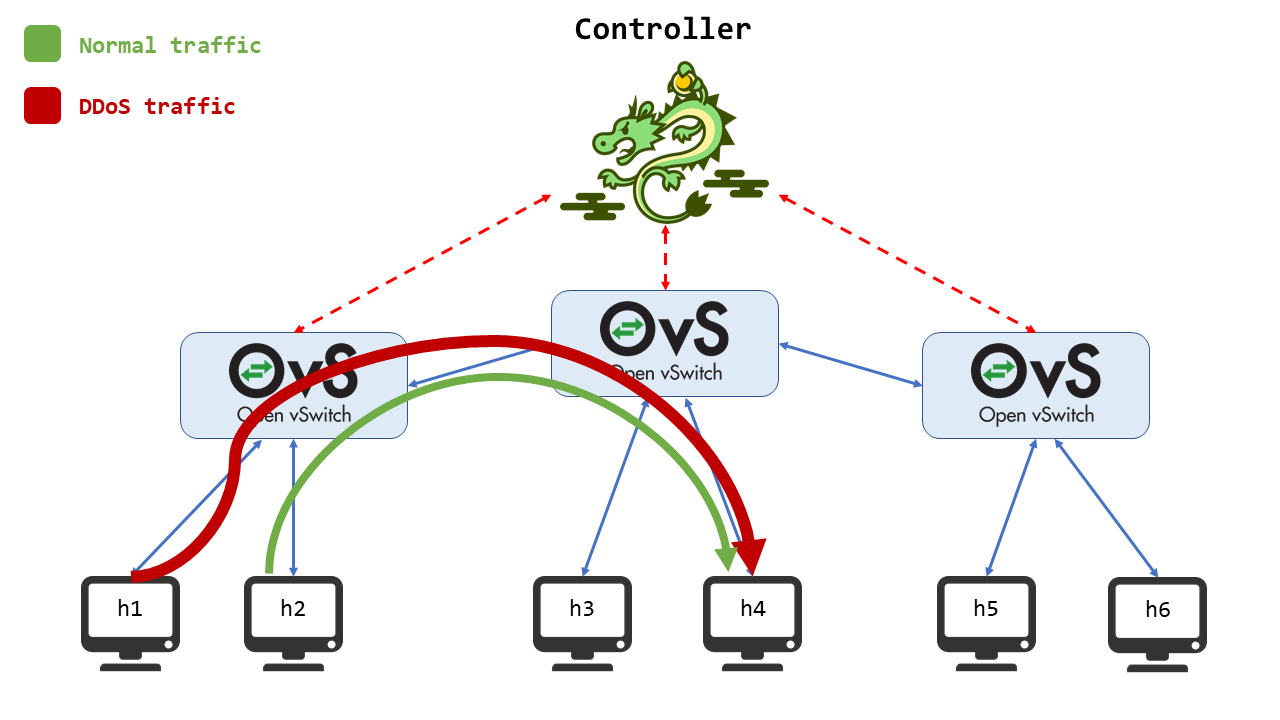
\includegraphics[scale = 1]{scenario_ddos.png}
				\caption{Under attack!}
				\label{f:dos_atk}
			\end{figure}

			Let's begin by setting up the scenario like we usually do:

			\begin{minted}{bash}
				sudo python3 scenario_basic.py
			\end{minted}

			Time to open terminals to both ICMP sources. We'll also fire up `Wireshark` on **Host4** to have a closer look at what's going on. Note the ampersand (`&`) at the end of the second command. It'll detach the `wireshark` process from the terminal so that we can continue running commands as we normally would. To do this we need to run:

			\begin{minted}{bash}
				mininet> xterm h1 h2
				mininet> h4 wireshark &
			\end{minted}

			Time to launch `hping3` from **Host1** with the parameters we discussed. This is shown in figure \ref{f:hpin3_ex}.

			\begin{figure}
				\centering
				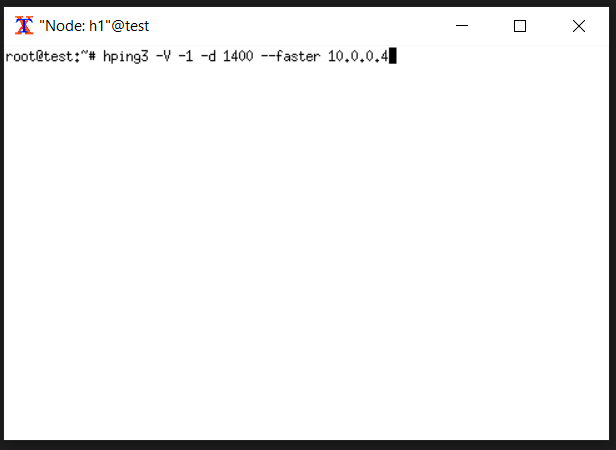
\includegraphics[scale = 1]{launch_hping3.png}
				\caption{Launching the \texttt{DoS} attack}
				\label{f:hping3_ex}
			\end{figure}

			If we now try to ping **Host4** from **Host2** we'll fail horribly as we find in figure \ref{f:net_down}.

			\begin{figure}
				\centering
				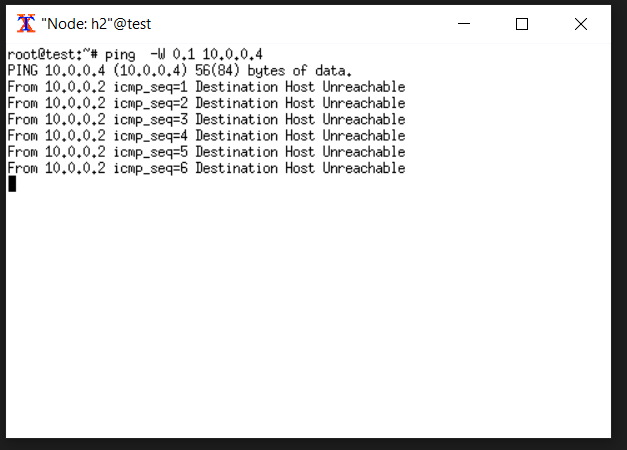
\includegraphics[scale = 1]{net_down.png}
				\caption{\textt{ICMP} traffic can't get through...}
				\label{f:net_down}
			\end{figure}

			If we halt the **DoS** attack we will see the regular traffic resume its normal operation after a short period of time. Figure \ref{f:net_ok} depicts this.

			\begin{figure}
				\centering
				\includegraphics[scale = 1]{net:ok.png}
				\caption{The network has recovered!}
				\label{f:net_ok}
			\end{figure}

			We then see how the **DoS** attack against **Host4** has been successful. In order to facilitate issuing the needed commands we have prepared a couple of `python` scripts containing all the needed information so that we only need to run them and be happy. You can find them at:

			\begin{itemize}
				\item Attack: \href{https://github.com/GAR-Project/project/blob/master/src/ddos.py}{`src/ddos.py`}
				\item Regular traffic: \href{https://github.com/GAR-Project/project/blob/master/src/normal.py}{`src/normal.py`}
			\enf{itemize}

			With all this ready to rock we now need to focus on detecting these attacks and seeing how to possibly mitigate them.

		\subsection{Wanted a Video}
			You can find a video showing the process we described step by step \href{https://www.youtube.com/watch?v=ofZPmV6_y_M}{here}. If you stumble upon any questions don't hesitate to contact us!


\end{document}